% SC4051 --- Chapter 3: RPC, Serialization and Messaging (0->100)
\chapter{Remote Calls, Serialization and Messaging}
\label{ch:rpc}

\begin{quote}
\emph{``Remote procedure call is the assembly language of distributed computing.''} --- Jim Waldo. It looks like a function call, but the network is between caller and callee, and that changes everything.
\end{quote}

\noindent\fbox{\parbox{\dimexpr\linewidth-2\fboxsep-2\fboxrule}{%
\textbf{From zero: from local calls to network calls.} We start with what a local call guarantees, add the network, and see why transparency is leaky. We then cover how data is encoded for the wire, how RPC is implemented, and when to use messaging instead. Every idea is grounded in runnable Python.}}
\vspace{0.4em}

\section*{Learning Outcomes}
After this chapter you will be able to:
\begin{enumerate}[label=(L\arabic*)]
    \item explain why RPC cannot be fully transparent (partial failure, latency, at-most/at-least/exactly-once);
    \item compare serialization formats (JSON, Protocol Buffers, Avro) on schema evolution and efficiency;
    \item describe gRPC/Thrift stub generation and streaming modes;
    \item contrast RPC (request--reply) with message queues and pub/sub on coupling and durability;
    \item implement idempotency keys and retry budgets to achieve effective exactly-once.
\end{enumerate}

% ============================================================
\section{From Local Calls to Remote Calls}
\label{sec:local-vs-remote}
A local call is \emph{total}: it either returns a value or raises an exception, and failure means the whole process failed. A remote call can fail \emph{partially}: the request was sent but the reply was lost, so the caller does not know whether the callee executed. This is the fundamental transparency break.

Wal\-do et al.\ (1994) argued RPC can never be fully transparent because objects differ in failure, latency, memory access and concurrency. Hiding the network behind the same syntax invites fallacy~1 and~2 (Ch.~1) into application code.

\begin{figure}[h]
\centering
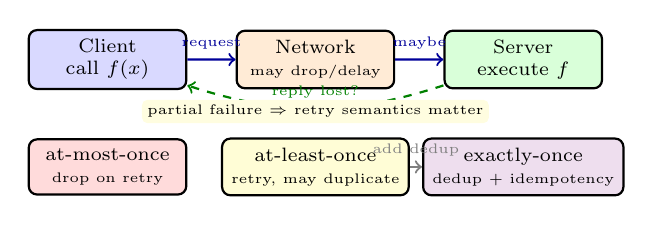
\begin{tikzpicture}[scale=0.88, every node/.style={font=\scriptsize},
  box/.style={draw,rounded corners=3pt,minimum width=2.0cm,minimum height=0.70cm,align=center,thick}]
\node[box,fill=blue!15] (client) at (0,1.7) {Client\\call $f(x)$};
\node[box,fill=orange!16] (net) at (3.0,1.7) {Network\\{\tiny may drop/delay}};
\node[box,fill=green!15] (server) at (6.0,1.7) {Server\\execute $f$};
\node[box,fill=red!14] (a) at (0,0.15) {at-most-once\\{\tiny drop on retry}};
\node[box,fill=yellow!16] (b) at (3.0,0.15) {at-least-once\\{\tiny retry, may duplicate}};
\node[box,fill=violet!13] (c) at (6.0,0.15) {exactly-once\\{\tiny dedup + idempotency}};
\draw[->,thick,blue!60!black] (client) -- (net) node[midway,above,font=\tiny] {request};
\draw[->,thick,blue!60!black] (net) -- (server) node[midway,above,font=\tiny] {maybe};
\draw[->,thick,green!50!black,dashed] (server) to[bend left=18] node[midway,above,font=\tiny] {reply lost?} (client);
\draw[->,thick,gray] (b) -- (c) node[midway,above,font=\tiny] {add dedup};
\node[font=\tiny,fill=yellow!12,rounded corners=2pt,inner sep=2pt] at (3.0,0.95) {partial failure $\Rightarrow$ retry semantics matter};
\end{tikzpicture}
\caption{RPC partial failure: did the server run $f$? The answer determines at-most vs.\ at-least vs.\ effective exactly-once.}
\label{fig:rpc-partial}
\end{figure}

\paragraph{Retry semantics.}
\begin{description}[leftmargin=1.2em,style=nextline]
    \item[At-most-once] Send once; on timeout return error. Safe against duplication but loses operations.
    \item[At-least-once] Retry until ack; may execute multiple times. Requires idempotent handler or deduplication.
    \item[Exactly-once (effective)] At-least-once + server-side dedup via idempotency key + idempotent side effects. True exactly-once over an unreliable network is impossible in general; this is the practical approximation.
\end{description}

\begin{definition}[Idempotency]
An operation $f$ is \emph{idempotent} if $f(f(x))=f(x)$: repeating it has the same effect as doing it once. Example: $x:=5$ is idempotent; $x{+}{+}$ is not. Non-idempotent operations need an idempotency key so the server can recognise retries.
\end{definition}

% ============================================================
\section{Serialization and Interface Definition}
\label{sec:serial}
Before bytes go on the wire they must be \emph{serialized} (marshalled). Choices trade readability, size, speed and schema evolution.

\begin{table}[h]
\centering\small
\begin{tabular}{lcccc}
\toprule
Format & Human-readable & Size & Schema & Evolution \\
\midrule
JSON & yes & large & none & ad-hoc \\
XML & yes & larger & XSD & verbose \\
Protocol Buffers & no & small & .proto & excellent (field tags) \\
Avro & no & small & JSON schema & excellent (reader/writer) \\
Thrift & no & small & .thrift & good \\
\bottomrule
\end{tabular}
\caption{Serialization trade-offs. Binary IDLs win on size and evolution; JSON wins on debugging.}
\label{tab:serial}
\end{table}

\paragraph{Schema evolution rules.} Adding a field must not break old readers (use optional with defaults); removing a field must reserve its tag; changing a type is often incompatible. Protobuf's field numbers and Avro's reader/writer schemas exist precisely to make evolution safe---JSON's flexibility is also its danger (silent missing-field bugs).

\begin{lstlisting}[language=Python]
# Serialization comparison: JSON vs Protobuf-style varint (illustrative)
import json, struct

# JSON: readable but verbose, no schema enforcement
payload = {"user_id": 42, "action": "deposit", "amount": 100}
json_bytes = json.dumps(payload).encode()
print("JSON bytes:", len(json_bytes), json_bytes[:40])

# Simulated protobuf varint for an integer field (LEB128)
def varint_encode(n):
    out = bytearray()
    while n >= 0x80:
        out.append((n & 0x7F) | 0x80)
        n >>= 7
    out.append(n)
    return bytes(out)

for v in [1, 127, 128, 300, 10_000]:
    print(f"{v:6d} -> varint {varint_encode(v).hex()} ({len(varint_encode(v))}B)")

# Idempotency key pattern: server deduplicates by key
store = {}
def handle_request(key, op):
    if key in store:          # duplicate retry
        return store[key]
    result = op()             # execute once
    store[key] = result
    return result
\end{lstlisting}

\begin{figure}[h]
\centering
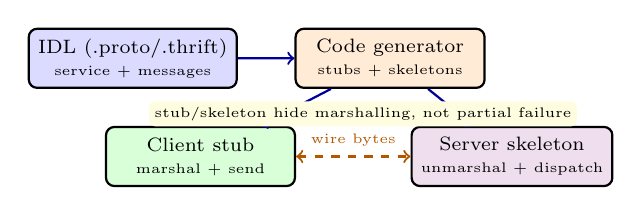
\begin{tikzpicture}[scale=0.86, every node/.style={font=\scriptsize},
  box/.style={draw,rounded corners=3pt,minimum width=2.4cm,minimum height=0.75cm,align=center,thick}]
\node[box,fill=blue!14] (idl) at (0,1.6) {IDL (.proto/.thrift)\\{\tiny service + messages}};
\node[box,fill=orange!16] (gen) at (3.8,1.6) {Code generator\\{\tiny stubs + skeletons}};
\node[box,fill=green!15] (cli) at (1.0,0.15) {Client stub\\{\tiny marshal + send}};
\node[box,fill=violet!13] (srv) at (5.6,0.15) {Server skeleton\\{\tiny unmarshal + dispatch}};
\draw[->,thick,blue!60!black] (idl) -- (gen);
\draw[->,thick,blue!60!black] (gen) -- (cli);
\draw[->,thick,blue!60!black] (gen) -- (srv);
\draw[<->,thick,orange!70!black,dashed] (cli) -- (srv) node[midway,above,font=\tiny] {wire bytes};
\node[font=\tiny,fill=yellow!12,rounded corners=2pt,inner sep=2pt] at (3.4,0.78) {stub/skeleton hide marshalling, not partial failure};
\end{tikzpicture}
\caption{IDL-driven RPC: the interface definition generates client stubs and server skeletons; the wire format is fixed by the IDL compiler.}
\label{fig:idl}
\end{figure}

% ============================================================
\section{gRPC, Thrift and Streaming}
\label{sec:grpc}
Modern RPC frameworks share a pattern: define the service in an IDL, generate code, run over HTTP/2 or a custom transport.

\paragraph{gRPC (Protobuf + HTTP/2).} Four modes: unary (one request, one response), server-streaming, client-streaming, bidirectional streaming. HTTP/2 multiplexing, flow control and header compression come for free. Interceptors provide auth, tracing and retry budgets.

\paragraph{Thrift (Apache).} Similar IDL with multiple transports (framed, header) and protocols (binary, compact, JSON). Widely used at Meta.

Streaming matters because \emph{not every interaction is request--reply}. A log tail or price feed is naturally a stream; polling it via unary RPC wastes latency and load.

\begin{lstlisting}[language=Python]
# Retry with idempotency key and exponential backoff + jitter (client side)
import random, time, uuid

def rpc_with_retry(stub_call, max_retries=4, base_ms=50):
    key = str(uuid.uuid4())          # idempotency key reused across retries
    for attempt in range(max_retries + 1):
        try:
            return stub_call(idempotency_key=key)
        except TimeoutError:
            if attempt == max_retries:
                raise
            # exponential backoff with jitter avoids thundering herd
            sleep_ms = base_ms * (2 ** attempt) + random.randint(0, 30)
            time.sleep(sleep_ms / 1000.0)
    # Server: if key seen before, return cached response (see earlier handle_request)

# Example: safe retry of a payment (non-idempotent without key)
def make_payment(amount):
    def call(key=None):
        # stub would send key in header; server deduplicates
        return f"charged {amount} (key={key[:8]}...)"
    return rpc_with_retry(lambda idempotency_key: call(idempotency_key))

print(make_payment(50))
\end{lstlisting}

\begin{figure}[h]
\centering
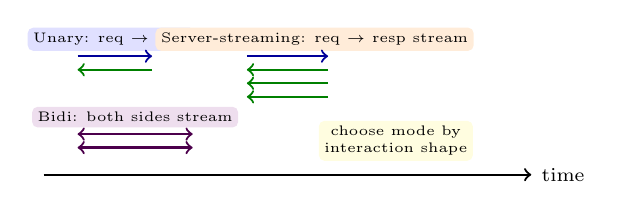
\begin{tikzpicture}[scale=0.86, every node/.style={font=\scriptsize}]
\draw[->,thick] (0,0) -- (7.2,0) node[right] {time};
% Unary
\node[font=\tiny,fill=blue!12,rounded corners=2pt,inner sep=2pt] at (1.0,2.0) {Unary: req $\to$ resp};
\draw[->,blue!60!black,thick] (0.5,1.75) -- (1.6,1.75);
\draw[->,green!50!black,thick] (1.6,1.55) -- (0.5,1.55);
% Server streaming
\node[font=\tiny,fill=orange!15,rounded corners=2pt,inner sep=2pt] at (4.0,2.0) {Server-streaming: req $\to$ resp stream};
\draw[->,blue!60!black,thick] (3.0,1.75) -- (4.2,1.75);
\draw[->,green!50!black,thick] (4.2,1.55) -- (3.0,1.55);
\draw[->,green!50!black,thick] (4.2,1.35) -- (3.0,1.35);
\draw[->,green!50!black,thick] (4.2,1.15) -- (3.0,1.15);
% Bidi
\node[font=\tiny,fill=violet!13,rounded corners=2pt,inner sep=2pt] at (1.35,0.85) {Bidi: both sides stream};
\draw[<->,violet!60!black,thick] (0.5,0.60) -- (2.2,0.60);
\draw[<->,violet!60!black,thick] (0.5,0.40) -- (2.2,0.40);
\node[font=\tiny,align=center,fill=yellow!12,rounded corners=2pt,inner sep=2pt] at (5.2,0.50) {choose mode by\\interaction shape};
\end{tikzpicture}
\caption{gRPC interaction modes. Streaming avoids polling when data flows continuously.}
\label{fig:grpc-modes}
\end{figure}

% ============================================================
\section{Messaging: Queues and Pub/Sub}
\label{sec:messaging}
RPC couples caller and callee in time (both must be up) and space (caller knows callee). Messaging decouples them.

\begin{description}[leftmargin=1.2em,style=nextline]
    \item[Message queue (point-to-point)] Producer sends to a queue; one consumer receives. Durable queues (RabbitMQ, SQS, Kafka with consumer groups) survive consumer failure and smooth bursts. Semantics: at-least-once delivery, ordering per partition.
    \item[Publish/subscribe] Publisher sends to a topic; many subscribers receive. Decouples publishers from subscriber count (Kafka, SNS, Redis Pub/Sub). Ordering is per topic-partition, not global.
    \item[Log (Kafka-style)] An append-only partitioned log that is both queue and pub/sub: consumers track offsets, replay is possible, retention is time/size-based. The log is the database.
\end{description}

When to use which: RPC for request--reply with low latency and strong typing; queues for work distribution and back-pressure; pub/sub for event broadcast and fan-out; logs when you need replay and audit. Many architectures mix them: an API gateway speaks gRPC to clients and publishes domain events to Kafka for downstream consumers.

\begin{example}[Ordering pitfall]
Two producers send $A$ then $B$ to different Kafka partitions. A consumer reading both partitions may see $B$ before $A$. If order matters, the producer must key both messages to the same partition (same key $\to$ same partition $\to$ total order per key).
\end{example}

% ============================================================
\section{Exercises}
\label{sec:ch03-exercises}
\begin{enumerate}[label=E3.\arabic*, leftmargin=*, itemsep=0.6em]
    \item \textbf{Partial failure analysis.} A client sends RPC $pay(\$100)$ and times out. Enumerate the four possible server states (never received, executed but reply lost, executed and reply in flight, failed before execution). For each, state whether retrying is safe without an idempotency key.
    \item \textbf{Schema evolution.} A Protobuf message has fields $1{:}user\_id$, $2{:}email$. You need to rename $email$ to $contact\_email$ and add $phone$. Show the .proto diff that is wire-compatible with old binaries. What breaks if you reuse field number 2 for $phone$?
    \item \textbf{Retry budgets.} A service at 1000\,RPS has a 1\% timeout rate. With blind retry (one retry per timeout), compute the extra load during a 10\% timeout spike. Propose a retry budget (e.g., 20\% of requests) and explain how it prevents retry storms.
    \item \textbf{RPC vs.\ messaging.} Design the interaction for an image-upload service that must (a) return upload success quickly and (b) generate thumbnails asynchronously. Justify using RPC for (a) and a queue/log for (b). Where does ordering matter and how would you guarantee it?
    \item \textbf{Exactly-once simulation.} Extend the idempotency-key handler in the chapter's Python to persist the dedup table to disk (crash-recovery model). Show a trace where the server crashes after executing but before acking, restarts, and correctly deduplicates the client's retry.
\end{enumerate}

% ============================================================
\section*{Chapter Notes}
Waldo et al., ``A note on distributed computing'' (1994) is the classic transparency critique. Birrell--Nelson (1984) introduced RPC. gRPC: \texttt{grpc.io}; Thrift: Apache Thrift whitepaper (2007). Serialization evolution: Kleppmann, \emph{Designing Data-Intensive Applications}, Ch.~4 (2017) is the best single reference. Messaging semantics and Kafka logs: Kleppmann Ch.~11 and Kreps, ``The Log'' (2013).

% End of Chapter 3
